\documentclass[11pt,a4paper]{article}

\usepackage[utf8]{inputenc}
\usepackage[T1]{fontenc}
\usepackage{lmodern}
\usepackage{microtype}
\usepackage[margin=2.5cm]{geometry}
\usepackage{graphicx}
\usepackage{booktabs}
\usepackage{tabularx}
\usepackage{caption}
\usepackage{xcolor}
\usepackage{tikz}
\usetikzlibrary{positioning,arrows.meta}
\usepackage[numbers,sort&compress]{natbib}
\usepackage[hidelinks]{hyperref}

\captionsetup{font=small,labelfont=bf}
\graphicspath{{../results/figures/}}
\newcolumntype{Y}{>{\raggedright\arraybackslash}X}

\title{Student Well-Being and Mental Health Analytics:\\
A Systematic Review and Comparative Bibliometric Analysis of\\
IEEE Xplore, ScienceDirect and SpringerLink (2021--2026)}
\author{Cristhian Eduardo Osorio Restrepo\\[2pt]
\small ORCID: \href{https://orcid.org/0009-0004-6899-4555}{\texttt{0009-0004-6899-4555}}\\
\small Universidad del Quindío, Colombia\\
\small \href{mailto:cristhiane.osorior@uqvirtual.edu.co}{\texttt{cristhiane.osorior@uqvirtual.edu.co}} (institutional)\\
\small \href{mailto:osoriocristhian86@gmail.com}{\texttt{osoriocristhian86@gmail.com}} (secondary)}
\date{}

\begin{document}
\maketitle

% =====================================================================
\begin{abstract}
Student well-being and mental health analytics applies data analytics, data mining and machine learning to data about students in order to assess, predict or monitor their mental health and well-being. This study combines a systematic review of abstracts with a comparative bibliometric analysis of the research on this topic published between 2021 and 2026 in IEEE Xplore, ScienceDirect and SpringerLink. Metadata for 1072 records with abstracts were retrieved through the official APIs of the three databases, and every abstract was screened and coded with a closed codebook. Of these records, 336 were unrelated to the topic, 230 were excluded after review, 4 were retracted and 502 were retained (426 from IEEE Xplore, 33 from ScienceDirect and 43 from SpringerLink). The retained studies are mostly predictive models (65\%) about university students (66\%), focused on stress (32\%), depression (27\%) and anxiety (20\%), and built mainly with classical classifiers and tree ensembles. The share of studies that report explainable artificial intelligence rose from 4\% in 2021 to 32\% in 2026, and deep learning and natural language processing also grew. In IEEE Xplore, production grew at a compound annual rate of 59.1\% between 2021 and 2025 and is concentrated in India and China, with little international collaboration. Each database shows a different emphasis: predictive modelling in IEEE Xplore, the intersection of psychology and computing in ScienceDirect, and positive well-being constructs in SpringerLink. The abstracts also reveal methodological weaknesses: 39\% omit the data, the method or the result, at least 44 report performance values of 98\% or more, and only two report validation on an external cohort.
\end{abstract}

\noindent\textbf{Keywords:} student mental health; student well-being; learning analytics; machine learning; systematic review; bibliometric analysis

% =====================================================================
\section{Introduction}

Mental disorders are common among university students. In the World Health Organization (WHO) World Mental Health International College Student project, 31\% of 13{,}984 full-time first-year students from 19 colleges in 8 countries screened positive for at least one common mental disorder in the previous 12 months \cite{auerbach2018wmhicsp}. In the WHO World Mental Health Surveys, 20.3\% of college students had a 12-month disorder; 83.1\% of these cases began before university entry, and only 16.4\% of the students with a disorder received treatment \cite{auerbach2016college}.

Universities and researchers collect many kinds of data about students: questionnaires, academic records, smartphone and wearable sensor data, and text. Learning analytics is defined as the measurement, collection, analysis and reporting of data about learners and their contexts \cite{siemens2011analytics}, and machine learning provides methods to detect patterns and predict outcomes in mental health data \cite{shatte2019mlmh}. The StudentLife study, for example, found that passive smartphone sensing data were associated with the depression, stress and academic performance of college students \cite{wang2014studentlife}. In this paper, \emph{student well-being and mental health analytics} refers to the application of data analytics, data mining, machine learning or artificial intelligence to data about students in order to assess, predict or monitor their mental health or well-being.

A bibliometric analysis maps the structure and evolution of a research field from publication metadata \cite{donthu2021bibliometric,zupic2015bibliometric}, and a systematic review examines the content of the studies. \citet{demir2024aviation} combined both approaches to study artificial intelligence in aviation safety. This paper applies the same combination to student well-being and mental health analytics, with two differences: it analyses three databases separately instead of one, and it screens every abstract before the bibliometric analysis, so that the bibliometric maps describe only studies that belong to the topic.

The study addresses six research questions (RQ):

\begin{itemize}
  \item \textbf{RQ1:} How has scientific production on student well-being and mental health analytics evolved between 2021 and 2026?
  \item \textbf{RQ2:} Which countries produce this research, and how much do they collaborate internationally?
  \item \textbf{RQ3:} In which sources is this research published?
  \item \textbf{RQ4:} Which outcomes, populations, data sources and techniques concentrate the research?
  \item \textbf{RQ5:} How have the research topics changed over time?
  \item \textbf{RQ6:} What emphasis does each database show, and how do the databases differ?
\end{itemize}

Section~\ref{sec:method} describes the data collection, screening and analysis. Section~\ref{sec:review} presents the systematic review, Section~\ref{sec:biblio} the bibliometric analysis of each database and Section~\ref{sec:comparison} the comparison between databases. Section~\ref{sec:discussion} answers the research questions, Section~\ref{sec:limitations} states the limitations and Section~\ref{sec:conclusions} concludes.

% =====================================================================
\section{Methodology}\label{sec:method}

\subsection{Data sources and search strategy}

Metadata were retrieved through the official application programming interfaces (APIs) of three databases on 28 September 2026. The same search equation was expressed in the syntax of each API:

\begin{quote}\small
(student* OR ``higher education'' OR universit* OR college*) AND (``well-being'' OR wellbeing OR ``mental health'' OR ``psychological well-being'' OR ``emotional well-being'') AND (analytics OR ``learning analytics'' OR ``data analytics'' OR ``predictive analytics'' OR ``data mining'' OR ``machine learning'' OR ``big data''), publication years 2021--2026.
\end{quote}

IEEE Xplore was searched with the IEEE Xplore Metadata API in title, abstract and index terms. ScienceDirect records were retrieved through the Scopus Search API restricted to Elsevier-published documents (\texttt{TITLE-ABS-KEY}), because the ScienceDirect Search API requires an institutional token that was not available. SpringerLink was searched with the Springer Nature Meta API in the keyword field, because its free-text search matches full text and its title search is a paid feature. Missing fields (authors, affiliations, abstracts, citation counts and keywords) were completed from OpenAlex \cite{priem2022openalex} by DOI, without overwriting values provided by the source.

\subsection{Eligibility, screening and PRISMA flow}

Journal articles, conference papers and early access articles were retained, and duplicates were removed by normalised DOI and title. This produced 1165 records, of which 1072 had an abstract (933 from IEEE Xplore, 86 from ScienceDirect and 53 from SpringerLink).

Every abstract was then screened against the definition of the topic given in the introduction. A study was \emph{included} only if the outcome it analyses or predicts is the mental health or well-being of students at any level of education. A study was \emph{excluded} when it was clearly unrelated to the topic, and \emph{doubtful} when its relevance was partial: the population was not clearly students; mental health or well-being was only a predictor of another outcome, such as academic performance, dropout or engagement; the outcome was a related but different construct, such as classroom environmental comfort, digital device use or opinions about courses or services; the study offered no data analysis; or the abstract was incoherent. Retracted articles were identified separately. Doubtful records were excluded from the synthesis and are reported as excluded after review. Figure~\ref{fig:prisma} shows the flow following PRISMA 2020 \cite{page2021prisma}.

Many retrieved records were unrelated to the topic. In IEEE Xplore, the share of records whose title mentions students or an educational setting fell from 94\% among the first 117 results to 9\% among the last 114. The API request set no sort order, and this pattern is consistent with results being returned by relevance, so the end of the list contains unrelated studies (for example, astronaut health monitoring or Parkinson's disease detection). In ScienceDirect, 42\% of the records were unrelated (for example, Alzheimer's disease imaging or glaucoma progression); the abstracts of several of these records mention a university or a ``wellbeing'' organisation in their affiliation or funding text, which the \texttt{TITLE-ABS-KEY} field matches.

\begin{figure}[htbp]
\centering
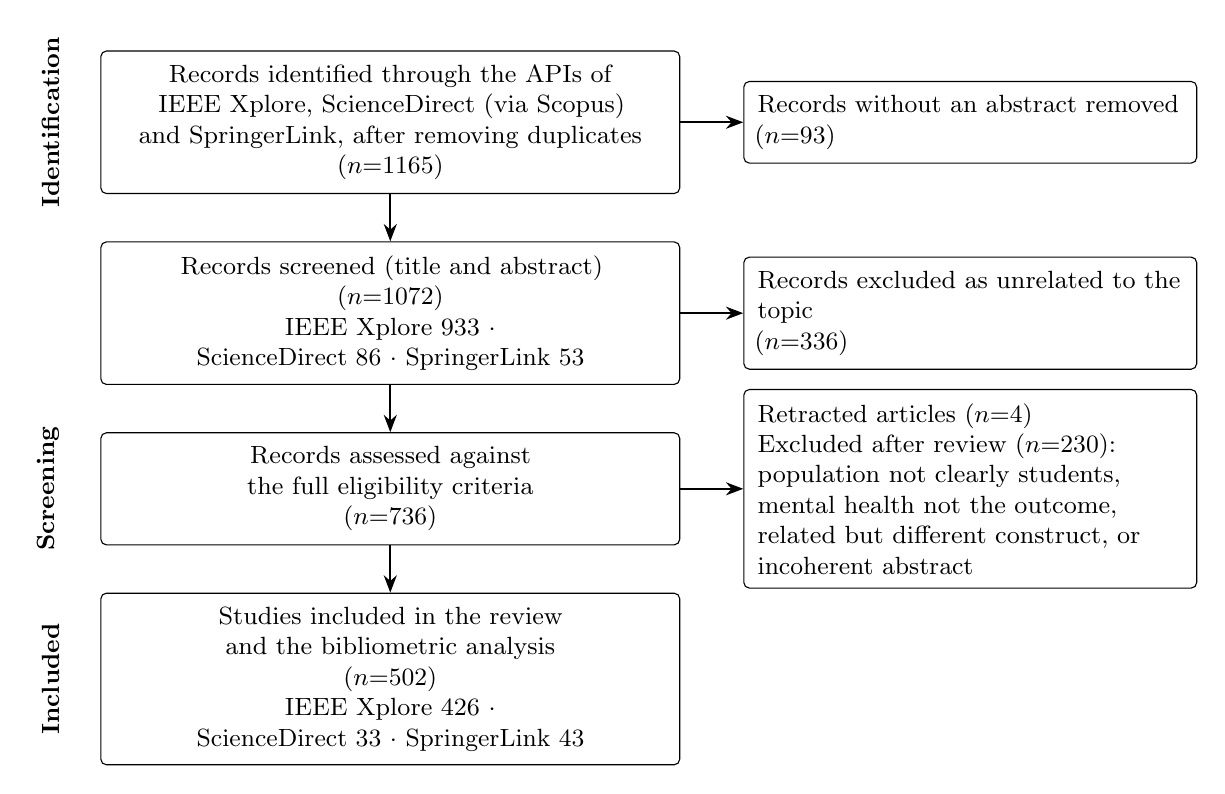
\begin{tikzpicture}[
  node distance=6mm and 8mm,
  box/.style={draw, rounded corners=2pt, align=center, text width=7cm, font=\small, inner sep=5pt, execute at begin node={\hyphenpenalty=10000}},
  side/.style={draw, rounded corners=2pt, align=left, text width=5.4cm, font=\small, inner sep=5pt, execute at begin node={\hyphenpenalty=10000}},
  lab/.style={font=\small\bfseries, rotate=90, anchor=south},
  arr/.style={-{Stealth[length=2.2mm]}, thick}]
  \node[box] (id) {Records identified through the APIs of IEEE Xplore, ScienceDirect (via Scopus) and SpringerLink, after removing duplicates\\ \mbox{($n{=}1165$)}};
  \node[box, below=of id] (scr) {Records screened (title and abstract)\\ \mbox{($n{=}1072$)}\\ IEEE Xplore 933 $\cdot$ \mbox{ScienceDirect 86} $\cdot$ \mbox{SpringerLink 53}};
  \node[box, below=of scr] (rev) {Records assessed against the full eligibility criteria\\ \mbox{($n{=}736$)}};
  \node[box, below=of rev] (inc) {Studies included in the review and the bibliometric analysis\\ \mbox{($n{=}502$)}\\ IEEE Xplore 426 $\cdot$ \mbox{ScienceDirect 33} $\cdot$ \mbox{SpringerLink 43}};
  \node[side, right=of id] (x0) {Records without an abstract removed\\ \mbox{($n{=}93$)}};
  \node[side, right=of scr] (x1) {Records excluded as unrelated to the topic\\ \mbox{($n{=}336$)}};
  \node[side, right=of rev] (x2) {Retracted articles \mbox{($n{=}4$)}\\ Excluded after review \mbox{($n{=}230$)}: population not clearly students, mental health not the outcome, related but different construct, or incoherent abstract};
  \draw[arr] (id) -- (scr); \draw[arr] (scr) -- (rev); \draw[arr] (rev) -- (inc);
  \draw[arr] (id) -- (x0); \draw[arr] (scr) -- (x1); \draw[arr] (rev) -- (x2);
  \node[lab] at ([xshift=-4mm]id.west) {Identification};
  \node[lab] at ([xshift=-4mm]rev.west) {Screening};
  \node[lab] at ([xshift=-4mm]inc.west) {Included};
\end{tikzpicture}
\caption{PRISMA 2020 flow diagram of record identification, screening and inclusion.}
\label{fig:prisma}
\end{figure}

\subsection{Data extraction}

Each abstract was coded with a closed codebook. The fields were: study type (predictive model, factor analysis, system or framework, review, descriptive), population (university, secondary school, vocational, mixed or unspecified), outcome (depression, anxiety, stress, suicide, general mental health risk, well-being, emotions, addiction, other), data source (survey, public dataset, large-scale survey such as PISA, institutional records, social media text, physiological sensors, smartphone, multimodal, not reported), method family (classical machine learning, ensembles and boosting, deep learning, reinforcement learning, natural language processing, association rules and clustering, statistical), use of explainable artificial intelligence (XAI), best reported result, country of the sample and a quality note. An abstract was marked \emph{vague} when it did not describe the data, the method or the result. A study could receive more than one value in a field, so percentages in Section~\ref{sec:review} can add up to more than 100\%. Only what the abstract states was coded. Coding conventions and every correction made after coding were documented in an audit log.

\subsection{Bibliometric analysis}

The bibliometric analysis was performed separately for each database on the included studies, with bibliometrix 5.5.0 in R \cite{aria2017bibliometrix}. It covers performance analysis (annual production, sources, countries and keywords) and science mapping (keyword co-occurrence networks, thematic maps and trend topics) \cite{donthu2021bibliometric}. Co-occurrence networks use the 40 most frequent keywords and the Louvain community detection algorithm \cite{blondel2008louvain}. Thematic maps place clusters obtained by co-word analysis \cite{callon1991coword} on a plane defined by centrality, the strength of a cluster's links with other clusters, and density, the strength of the links within the cluster \cite{cobo2011thematic}. Countries are counted for all authors (full counting), and a document is a multiple-country publication (MCP) when its authors come from more than one country.

Author keywords were used for IEEE Xplore and SpringerLink. The Scopus API does not return author keywords at the available access level, so the ScienceDirect analysis uses OpenAlex concepts, which are assigned automatically and describe broad disciplines rather than specific topics. Synonyms and spelling variants were unified with a thesaurus before the analysis. The APIs do not provide reference lists, so co-citation and bibliographic coupling could not be computed. Charts were kept only where the volume of data supports an interpretation; the charts excluded for each database, and the reasons, are stated in Section~\ref{sec:biblio}.

% =====================================================================
\section{Systematic Review of the Included Studies}\label{sec:review}

\subsection{Overview}

Table~\ref{tab:overview} summarises the 502 included studies. Most studies build predictive models (65\%), and about one in five describes a system or platform. The population is mainly university students (66\%); secondary school students appear in only 5\% of the studies. Stress (32\%), general mental health risk (30\%), depression (27\%) and anxiety (20\%) are the most studied outcomes, while positive well-being (10\%) and suicide (3\%) receive less attention. Questionnaires are the most frequent data source (34\%), and about one quarter of the abstracts (26\%) do not state what data were used.

\begin{table}[htbp]
\centering
\caption{Characteristics of the 502 included studies (a study can have more than one value per dimension).}
\label{tab:overview}
\small
\begin{tabularx}{\textwidth}{lY}
\toprule
Dimension & Distribution \\
\midrule
Study type & Predictive model 327 (65\%); system or framework 109 (22\%); factor analysis 42 (8\%); review 14 (3\%); descriptive 14 (3\%) \\
Population & University 331 (66\%); mixed or unspecified 141 (28\%); secondary school 27 (5\%); vocational 5 (1\%) \\
Outcome & Stress 163 (32\%); general mental health risk 149 (30\%); depression 135 (27\%); anxiety 102 (20\%); emotions 62 (12\%); well-being 50 (10\%); addiction 22 (4\%); suicide 14 (3\%) \\
Data source & Survey 169 (34\%); not reported 130 (26\%); multimodal 77 (15\%); physiological sensors 45 (9\%); public dataset 42 (8\%); smartphone 20 (4\%); social media text 18 (4\%); institutional records 11 (2\%); large-scale survey 9 (2\%) \\
Method family & Classical machine learning 218 (43\%); ensembles and boosting 199 (40\%); deep learning 154 (31\%); natural language processing 69 (14\%); statistical 59 (12\%); association rules and clustering 43 (9\%); reinforcement learning 4 (1\%); not reported 66 (13\%) \\
Explainability & XAI reported in 63 studies (13\%) \\
Abstract quality & Clear 307 (61\%); vague 195 (39\%) \\
\bottomrule
\end{tabularx}
\end{table}

\subsection{Thematic categories}

The included studies were grouped into eight thematic categories derived from the coded fields. The categories overlap, and 56 studies do not belong to any of them.

\paragraph{Prediction and screening of depression, anxiety and stress (229 studies, 46\%).} This is the largest category. These studies predict or classify depression, anxiety or stress, mostly from questionnaires, and compare several classifiers; 20\% of the abstracts in this category name a validated instrument such as the PHQ-9, GAD-7, PSS or DASS-21. Examples include the prediction of depression, anxiety and stress among university students in Lebanon during the 2024 war \cite{S001}, depression screening from daily habits in Bangladesh \cite{S011}, and the screening of anxiety, depression and burnout in 886 Swiss medical students \cite{I468}. Some studies use large samples, such as an explainable XGBoost model trained on 100{,}257 college students (AUC 0.887) \cite{S003} and a stacking ensemble trained on a public dataset of 27{,}901 students (AUC 0.919) \cite{D011}. Among the variables named in these abstracts, academic factors (pressure, workload or performance; 36\% of the abstracts), social support or family (14\%), sleep (14\%) and finances (8\%) appear most often. Bangladesh is the most frequent country stated in this category (23 studies).

\paragraph{Suicide risk (14 studies, 3\%).} Few studies address suicide directly. They predict suicidal ideation or behaviour from questionnaires, for example with a psychiatrist-validated dataset of 4004 students from 99 universities in Bangladesh (XGBoost, F1 75.4\%) \cite{S010}, a self-report instrument for medical students (SVM, AUC 0.81) \cite{I503}, and the WHO Global School-based Student Health Survey \cite{I820}.

\paragraph{Early warning systems and platforms (109 studies, 22\%).} These studies propose a complete system: a risk classifier embedded in a web or mobile application, a chatbot or an intervention engine. Examples are a mobile application that classifies medical students' stress from wearable physiological signals \cite{I388}, a sentiment-analysis chatbot that reformulates PHQ-9 items as open questions \cite{I212}, a chatbot based on cognitive behavioural therapy evaluated for usability with Peruvian students \cite{I476}, and a reinforcement learning agent that selects crisis interventions \cite{S004}. This category has the weakest reporting: 86 of the 109 abstracts are vague, and none reports the use of XAI.

\paragraph{Sensor-based and multimodal sensing (142 studies, 28\%).} These studies use wearables, smartphones or several data sources combined to capture behaviour and physiology. Examples include forecasting positive and negative affect one week ahead from wearable data combined with diaries \cite{D061}, interpretable models on the multi-year College Experience Study \cite{I089,I100}, an anxiety detection system based on sweat sensors evaluated on the StudentLife dataset \cite{D023}, and a multimodal framework tested on 14{,}604 students from 24 universities with external validation and fairness constraints \cite{S005}. Performance varies widely: a study that predicted subjective well-being from step count, heart rate and sleep reached 62\% accuracy \cite{D080}.

\paragraph{Language, text and emotion (109 studies, 22\%).} These studies analyse open-ended answers, diaries, social media posts or speech, or recognise emotions as indicators of mental state. Transformer models appear alongside classical classifiers, for example BERT and RoBERTa for classifying mental health conditions from students' texts \cite{I090,I254}. Machine learning, deep learning and language models combined with SHAP and LIME were applied to depression detection in Bangladeshi students \cite{D045}.

\paragraph{Positive well-being (50 studies, 10\%).} A smaller line of research treats well-being as a positive construct (life satisfaction, happiness, subjective and eudaimonic well-being) rather than as the absence of disorders. Three studies based on PISA data combine random forests or gradient boosting with hierarchical linear models, and all three identify school belonging among the strongest predictors, together with resilience, sense of meaning or fear of failure \cite{S040,S041,S048}. Other studies predict the happiness and life satisfaction of university students with external validation \cite{S021}, or relate health literacy and exercise adherence to the life satisfaction of 21{,}095 students \cite{D007}.

\paragraph{Addiction (22 studies, 4\%).} These studies predict behavioural addictions (internet, smartphone, gaming and social media) as mental health problems, for example in 3000 college students in China \cite{D063} and 569 engineering students \cite{I665}. Some report near-perfect performance, such as an R\textsuperscript{2} of 0.977 for nomophobia severity \cite{I344}.

\paragraph{Reviews (14 studies, 3\%).} The included reviews cover narrow subtopics, for example machine learning for stress detection in university students \cite{I192}, prediction of student stress and academic performance \cite{I501}, and machine learning with wearables and smartphones \cite{S049}. None of the 14 reviews reports a bibliometric analysis.

\subsection{Techniques by outcome}

Table~\ref{tab:methods} crosses method families with outcomes. Classical classifiers (logistic regression, support vector machines, decision trees, k-nearest neighbours, naive Bayes) and tree ensembles (random forests, gradient boosting, XGBoost, CatBoost) are the most frequent methods for depression, anxiety, stress and suicide. For emotions, where the input is often text, images or speech, deep learning (29 studies) and natural language processing (26) are more frequent than classical classifiers (12). In well-being research, statistical methods (13 of 50 studies) are almost as frequent as machine learning methods.

\begin{table}[htbp]
\centering
\caption{Number of included studies by outcome and method family (a study can use several methods and outcomes).}
\label{tab:methods}
\small
\setlength{\tabcolsep}{4pt}
\begin{tabular}{lrrrrrrr}
\toprule
Outcome & $n$ & Classical ML & Ensembles & Deep learning & NLP & Assoc./clust. & Statistical \\
\midrule
Stress & 163 & 85 & 65 & 54 & 27 & 3 & 15 \\
General MH risk & 149 & 46 & 33 & 44 & 22 & 29 & 16 \\
Depression & 135 & 70 & 78 & 48 & 12 & 6 & 13 \\
Anxiety & 102 & 47 & 45 & 39 & 14 & 7 & 15 \\
Emotions & 62 & 12 & 7 & 29 & 26 & 5 & 1 \\
Well-being & 50 & 16 & 18 & 9 & 7 & 4 & 13 \\
Addiction & 22 & 9 & 10 & 6 & 2 & 2 & 5 \\
Suicide & 14 & 9 & 7 & 2 & 1 & 0 & 1 \\
\bottomrule
\end{tabular}
\end{table}

\subsection{Evolution over time}

The content of the studies changed between 2021 and 2026 (Table~\ref{tab:years}). The share of studies using deep learning rose from 15\% in 2021 to 41\% in 2025, and the share reporting XAI methods such as SHAP \cite{lundberg2017shap} or LIME \cite{ribeiro2016lime} rose from 4\% in 2021 to 32\% in 2026. The share using natural language processing ranged between 7\% and 12\% until 2024 and reached 19\% in 2025. These changes agree with the keyword trends in Section~\ref{sec:biblio}, which are computed from metadata and not from the coded content.

\begin{table}[htbp]
\centering
\caption{Share of included studies per year using selected methods and data (2026 is a partial year).}
\label{tab:years}
\small
\begin{tabular}{lrrrrrr}
\toprule
 & 2021 & 2022 & 2023 & 2024 & 2025 & 2026 \\
\midrule
Studies ($n$) & 26 & 27 & 59 & 110 & 182 & 98 \\
XAI & 4\% & 4\% & 5\% & 6\% & 11\% & 32\% \\
Deep learning & 15\% & 19\% & 17\% & 29\% & 41\% & 30\% \\
Sensors, smartphone or multimodal data & 15\% & 26\% & 32\% & 29\% & 26\% & 33\% \\
Natural language processing & 12\% & 11\% & 7\% & 9\% & 19\% & 15\% \\
Positive well-being outcome & 4\% & 15\% & 14\% & 10\% & 12\% & 5\% \\
\bottomrule
\end{tabular}
\end{table}

\subsection{Methodological quality signals}

The abstracts show four weaknesses. First, 39\% of the abstracts are vague, and the share is much higher in IEEE Xplore (183 of 426, 43\%) than in SpringerLink (21\%) or ScienceDirect (9\%). Second, at least 44 of the 308 studies that report a performance value report 98\% or more, for example in samples of 520 to 1977 students \cite{S009,S033,D073}. Such values can indicate overfitting or information leakage between training and test data; small samples combined with inadequate validation are known to inflate performance estimates \cite{vabalas2019validation}, and leakage is a widespread cause of irreproducible machine learning results \cite{kapoor2023leakage}. Studies that report moderate results, such as accuracies between 0.57 and 0.69 for depression, anxiety and stress in 1697 students \cite{S025} or an AUC of about 0.52 for low well-being \cite{I186}, are less common. Third, only two abstracts report validation on an external cohort \cite{S005,S021}, and one more reports results on an independent validation set without describing its origin \cite{I857}; this is a lower bound, because other studies may report validation only in the full text. In the same way, fairness or bias is mentioned in 7 abstracts (1\%), calibration in 3 (1\%), and no abstract mentions a reporting guideline such as TRIPOD+AI \cite{collins2024tripodai}. Fourth, four retracted articles were found among the retrieved records, which shows that bibliometric corpora should be checked for retractions.

% =====================================================================
\section{Bibliometric Analysis}\label{sec:biblio}

\subsection{IEEE Xplore}

IEEE Xplore contributes 426 included documents (405 conference papers and 21 journal articles), 85\% of the total. Author keywords are available for 421 of them.

\paragraph{Annual production.} Production was 25 documents in 2021 and 24 in 2022, and then rose to 50 in 2023, 97 in 2024 and 160 in 2025 (Figure~\ref{fig:ieee-prod}), a compound annual growth rate of 59.1\% between 2021 and 2025. The 70 documents of 2026 cover only the period up to 28 September and are not comparable with full years.

\paragraph{Sources.} The literature is highly dispersed: the 426 documents appear in 342 sources, and the ten most productive sources hold only 42 documents (9.9\%) (Figure~\ref{fig:ieee-sources}). IEEE Access (12 documents) and IEEE Transactions on Affective Computing (4) are the only journals among them; the others are individual conference editions. The topic has no consolidated publication venue in IEEE Xplore.

\paragraph{Countries.} 402 documents have an identifiable country. India (153 documents, 38\%) and China (94, 23\%) lead, followed by Bangladesh (38), the United States (32) and Indonesia (22) (Figure~\ref{fig:ieee-countries}). Only 11.7\% of the documents have authors from more than one country. India (9\% MCP) and China (9\%) rarely publish with foreign partners, while the United States (56\%) and Oman (5 of 6 documents) publish mainly in collaboration. Peru (8 documents) is the only Latin American country among the ten most productive.

\paragraph{Keywords.} Machine learning appears in 44\% of the documents with keywords (187 of 421), followed by mental health (107) (Figure~\ref{fig:ieee-keywords}). Both are search terms, so their frequency partly reflects the query. The rest of the list is more informative: random forests (45), support vector machines (32) and decision trees (20) are as frequent as deep learning (28) and natural language processing (25), and explainable AI (27) is among the ten most frequent keywords. Depression (39), anxiety (29) and stress (24) are the most frequent conditions.

\paragraph{Co-occurrence network.} The 40 most frequent keywords form five clusters (Figure~\ref{fig:ieee-network}). The largest (red) links machine learning and mental health with the conditions (depression, anxiety, stress), the population (college and university students) and early intervention. The blue cluster groups the classical classifiers (random forests, support vector machines, decision trees, XGBoost, logistic regression, naive Bayes, k-nearest neighbours). The green cluster links student mental health with explainable AI, SHAP, SMOTE and depression detection. The purple cluster groups deep learning and convolutional neural networks with stress prediction and academic performance, and the orange cluster groups artificial intelligence, natural language processing, sentiment analysis, emotion recognition and chatbots.

\paragraph{Thematic map.} Machine learning, mental health and depression form a basic theme: high centrality and density close to the median (Figure~\ref{fig:ieee-thematic}). The classical classifiers (random forests, support vector machines, decision trees) have centrality slightly above the median and low density, in the area of basic themes. Student mental health with explainable AI and SHAP is a motor theme, both central and internally developed. Deep learning with convolutional neural networks and early intervention has the highest density and centrality just below the median, so it is a niche theme close to the motor themes. Stress management with machine learning algorithms and the internet of things is a niche theme with low centrality. Natural language processing with artificial intelligence and stress detection has low centrality and low density, the position of emerging or declining themes.

\paragraph{Trend topics.} The terms show a change over time (Figure~\ref{fig:ieee-trend}). Big data (median year 2022) and COVID-19 (2023) belong to the first years. Mental health, depression and support vector machines have their median in 2024, and machine learning, random forests and student mental health in 2025. The most recent terms (median 2026) are mental health prediction, depression prediction and wearable sensors. Because production grows every year, the median year of all terms tends towards recent years, so the relative order of the terms is more informative than the exact year.

\begin{figure}[htbp]
\centering
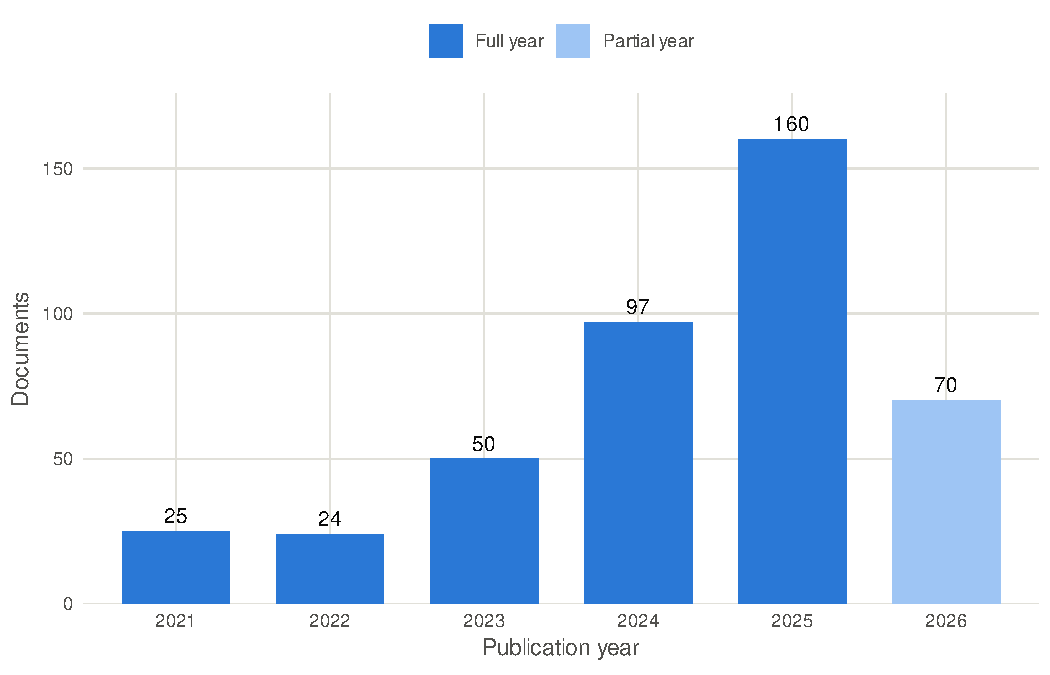
\includegraphics[width=0.75\textwidth]{ieee/en/01_annual_production}
\caption{IEEE Xplore: annual scientific production of included documents (2026 is a partial year, up to 28 September).}
\label{fig:ieee-prod}
\end{figure}

\begin{figure}[htbp]
\centering
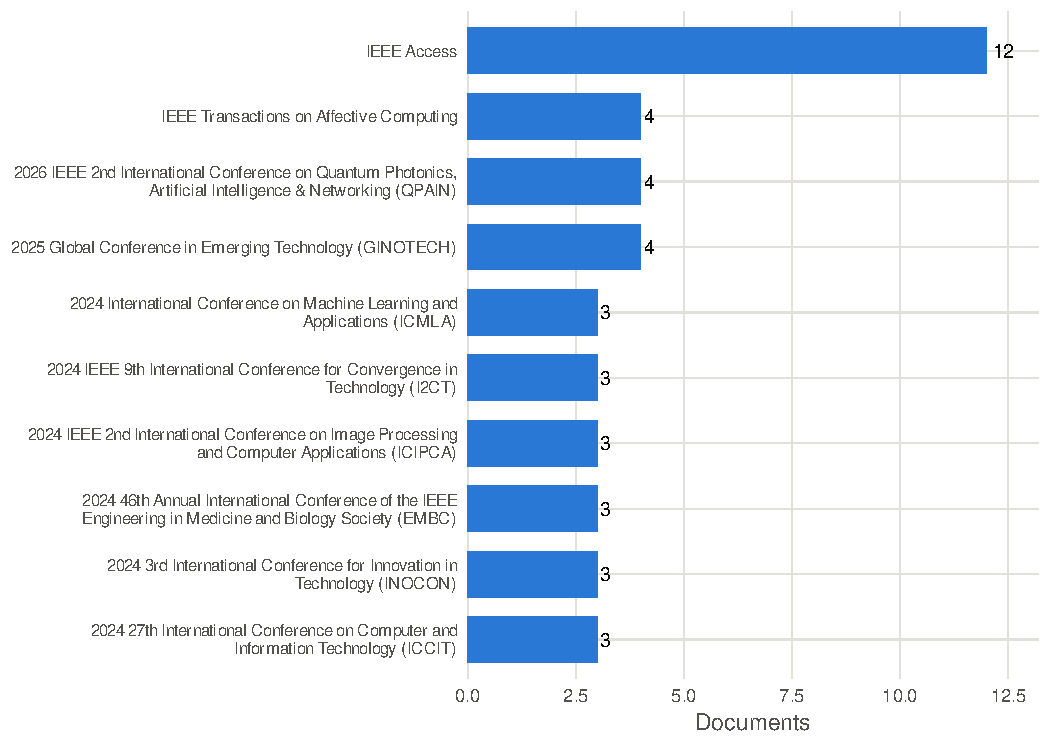
\includegraphics[width=0.85\textwidth]{ieee/en/02_sources}
\caption{IEEE Xplore: ten most relevant sources.}
\label{fig:ieee-sources}
\end{figure}

\begin{figure}[htbp]
\centering
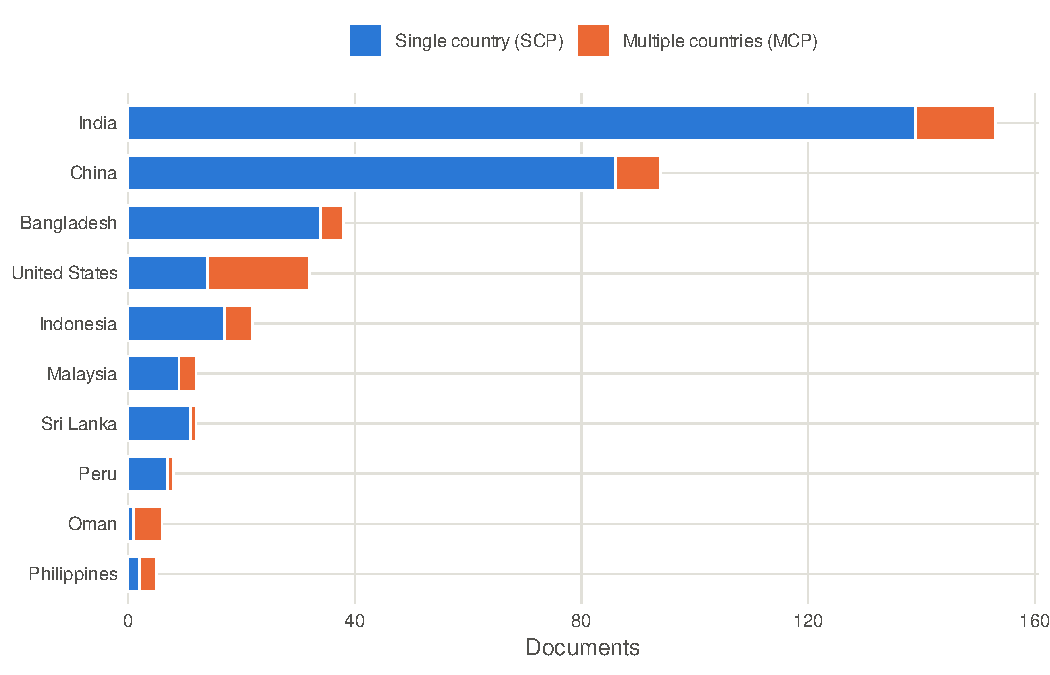
\includegraphics[width=0.75\textwidth]{ieee/en/03_countries}
\caption{IEEE Xplore: most productive countries (all authors, full counting), split into single-country (SCP) and multiple-country (MCP) publications.}
\label{fig:ieee-countries}
\end{figure}

\begin{figure}[htbp]
\centering
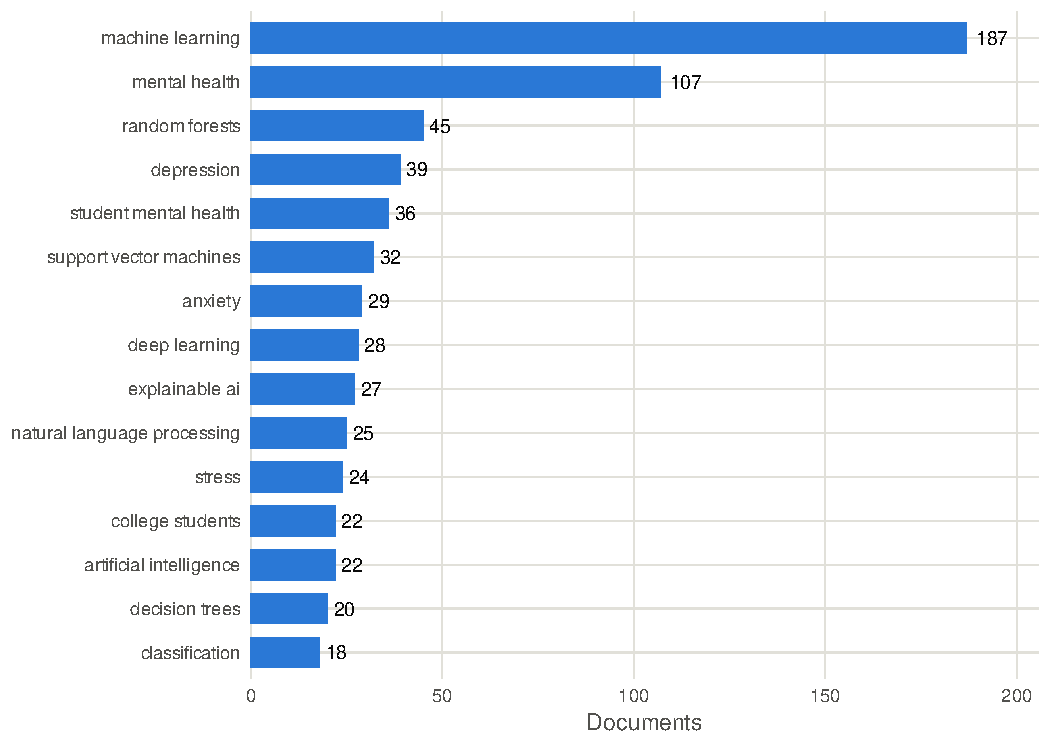
\includegraphics[width=0.75\textwidth]{ieee/en/04_keywords}
\caption{IEEE Xplore: most frequent author keywords.}
\label{fig:ieee-keywords}
\end{figure}

\begin{figure}[htbp]
\centering
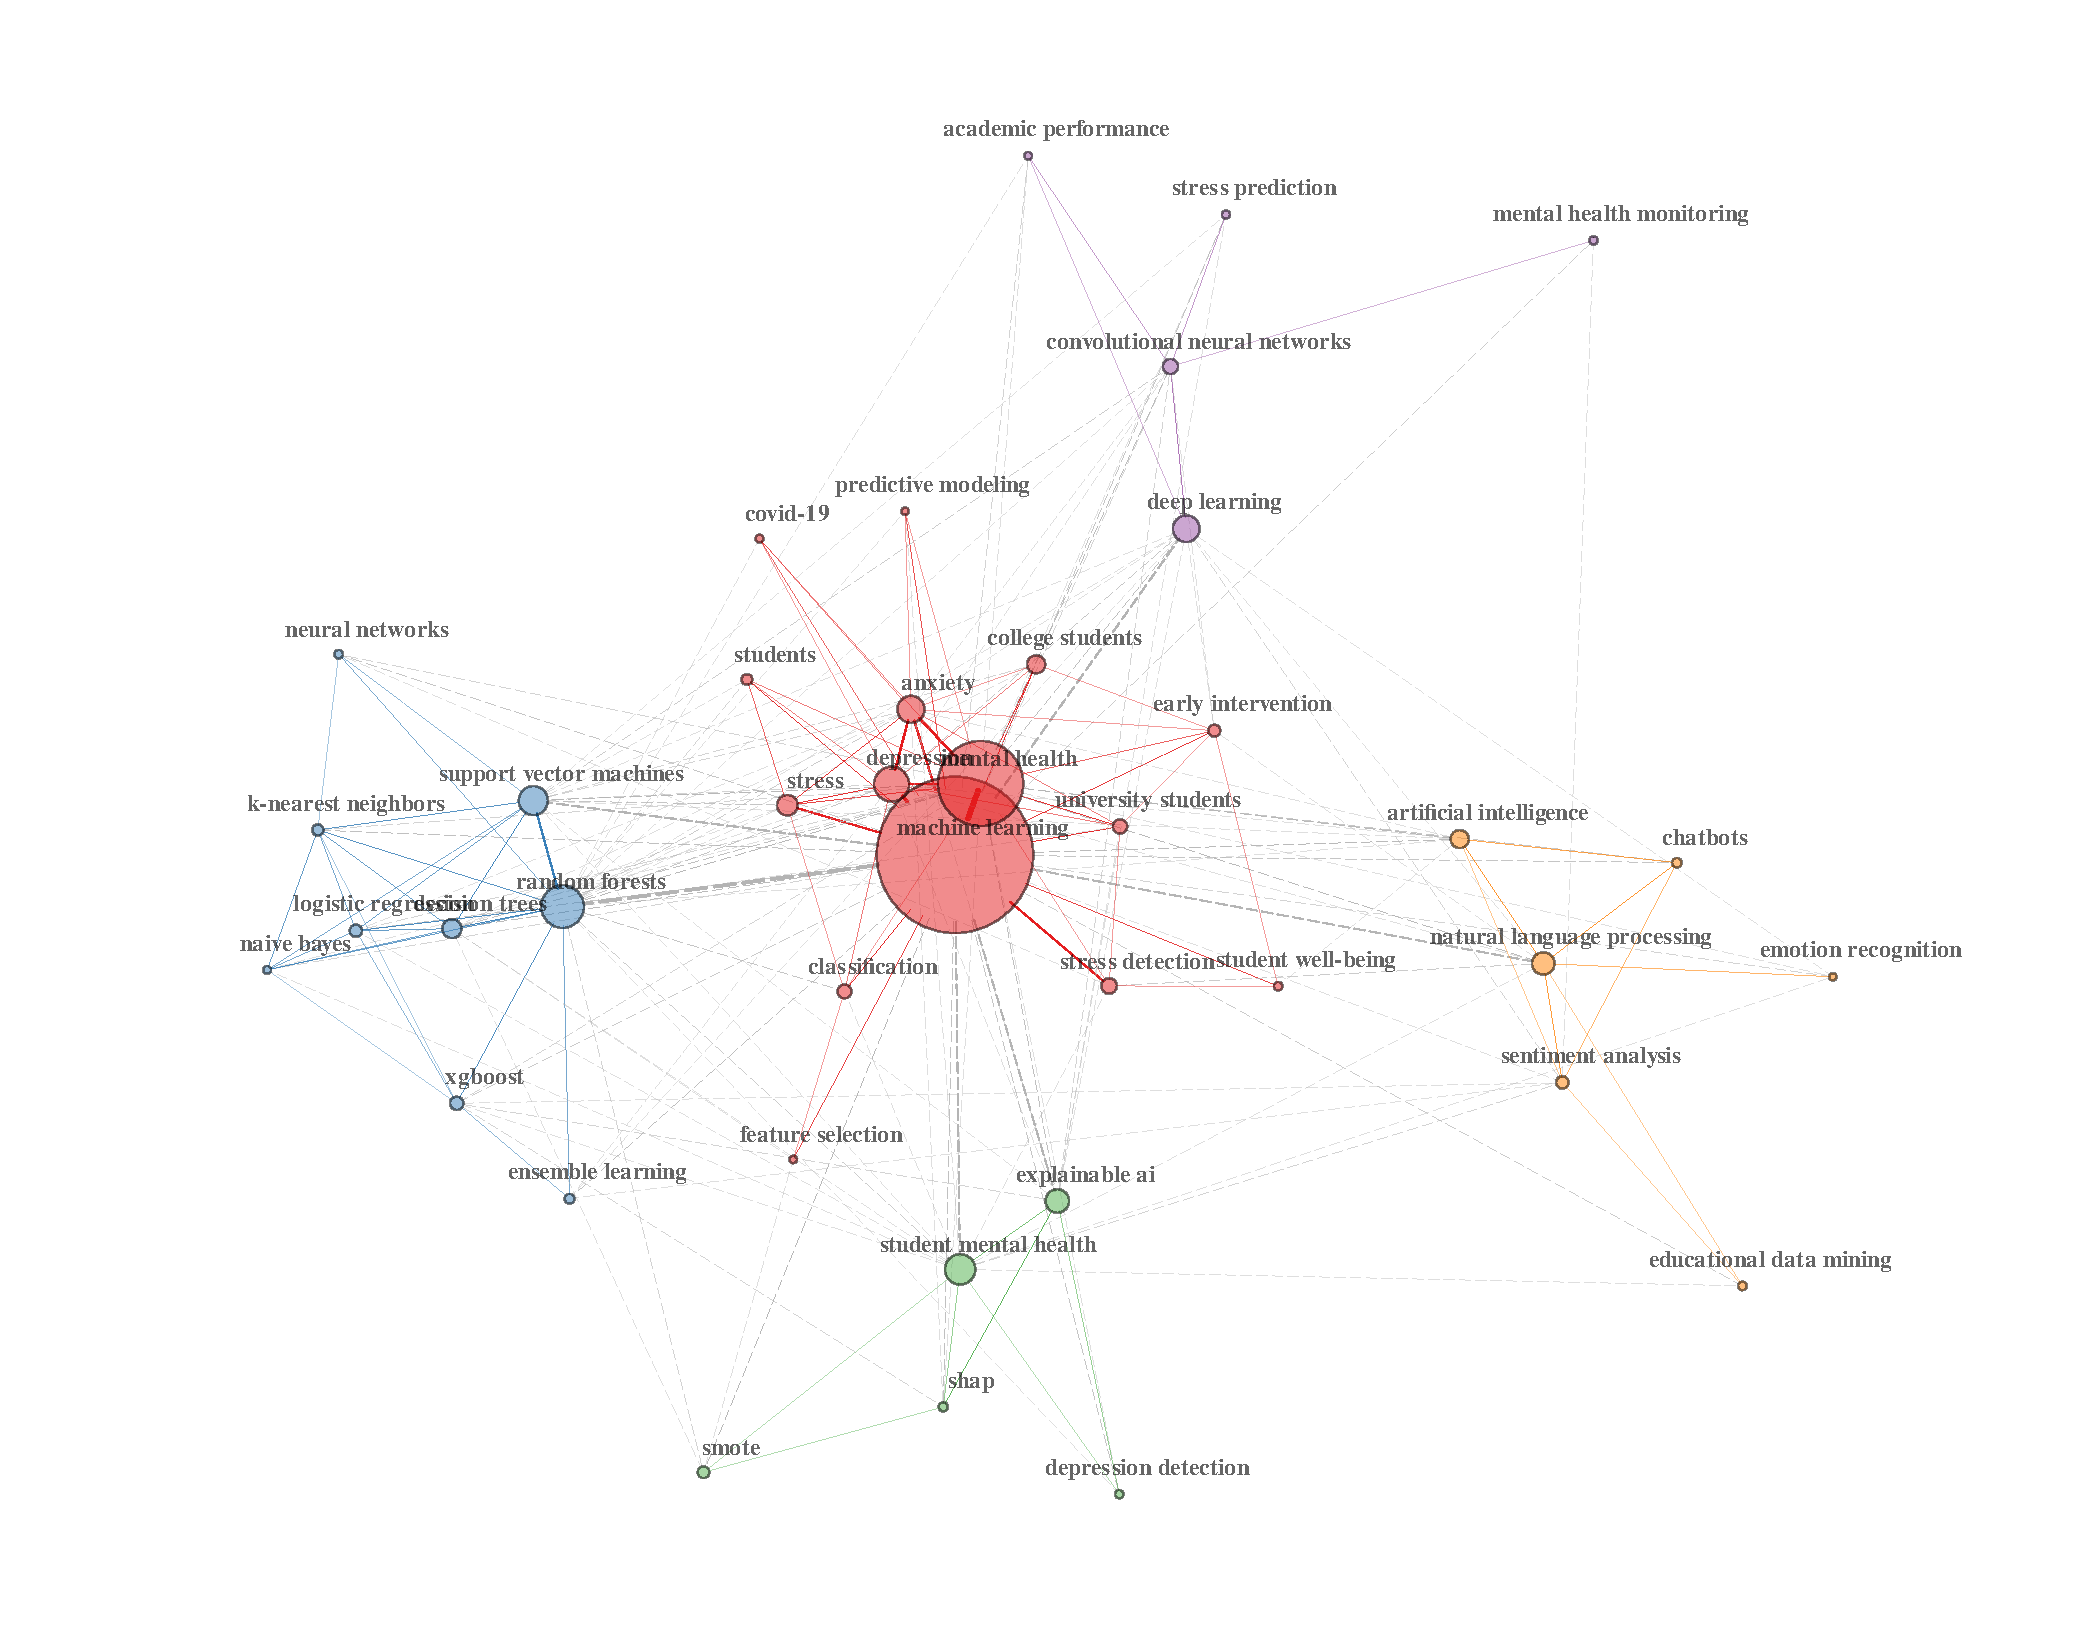
\includegraphics[width=\textwidth]{ieee/en/05_cooccurrence_network}
\caption{IEEE Xplore: co-occurrence network of the 40 most frequent author keywords (Louvain clusters).}
\label{fig:ieee-network}
\end{figure}

\begin{figure}[htbp]
\centering
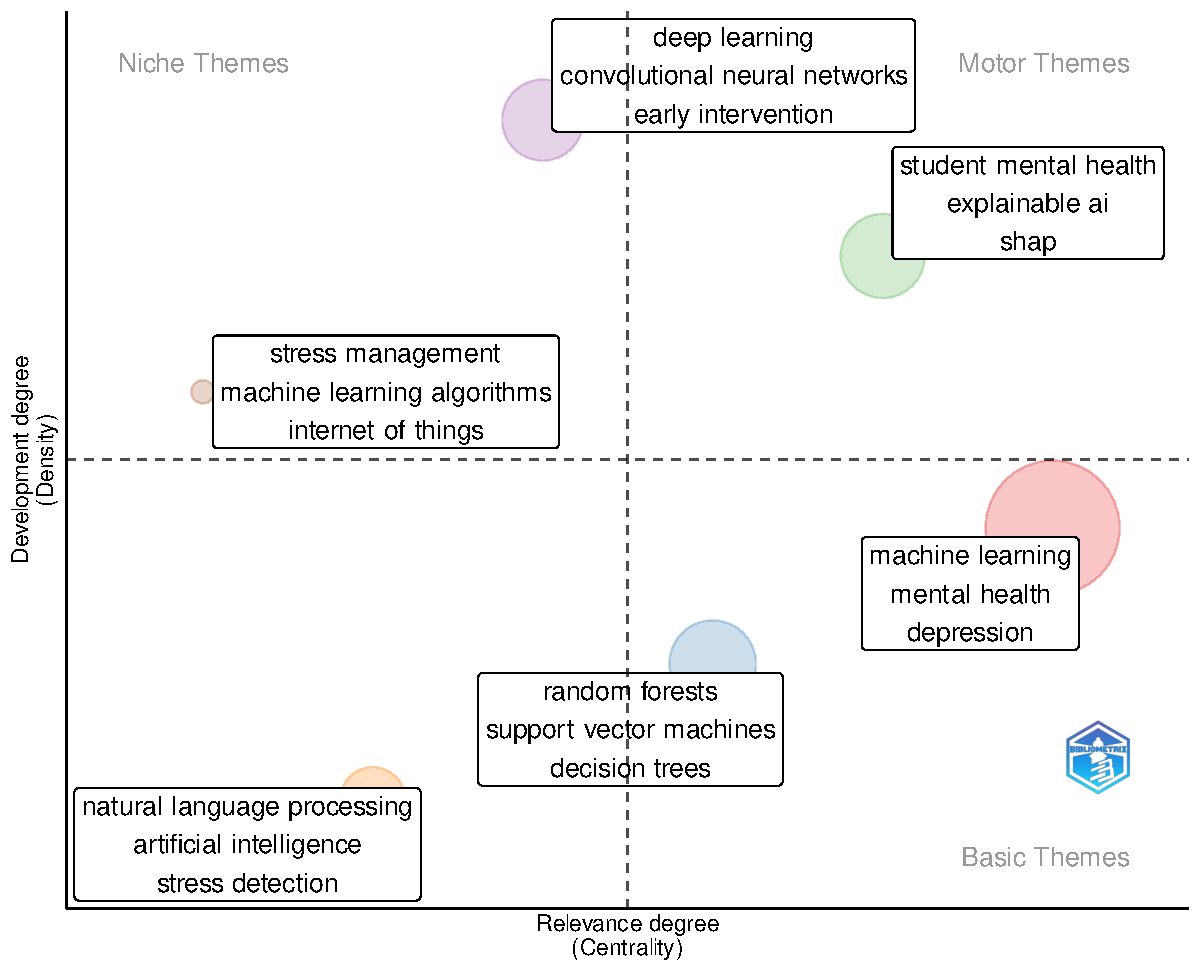
\includegraphics[width=0.85\textwidth]{ieee/en/06_thematic_map}
\caption{IEEE Xplore: thematic map of author keywords (centrality versus density). Quadrants: motor themes (upper right), niche themes (upper left), emerging or declining themes (lower left) and basic themes (lower right).}
\label{fig:ieee-thematic}
\end{figure}

\begin{figure}[htbp]
\centering
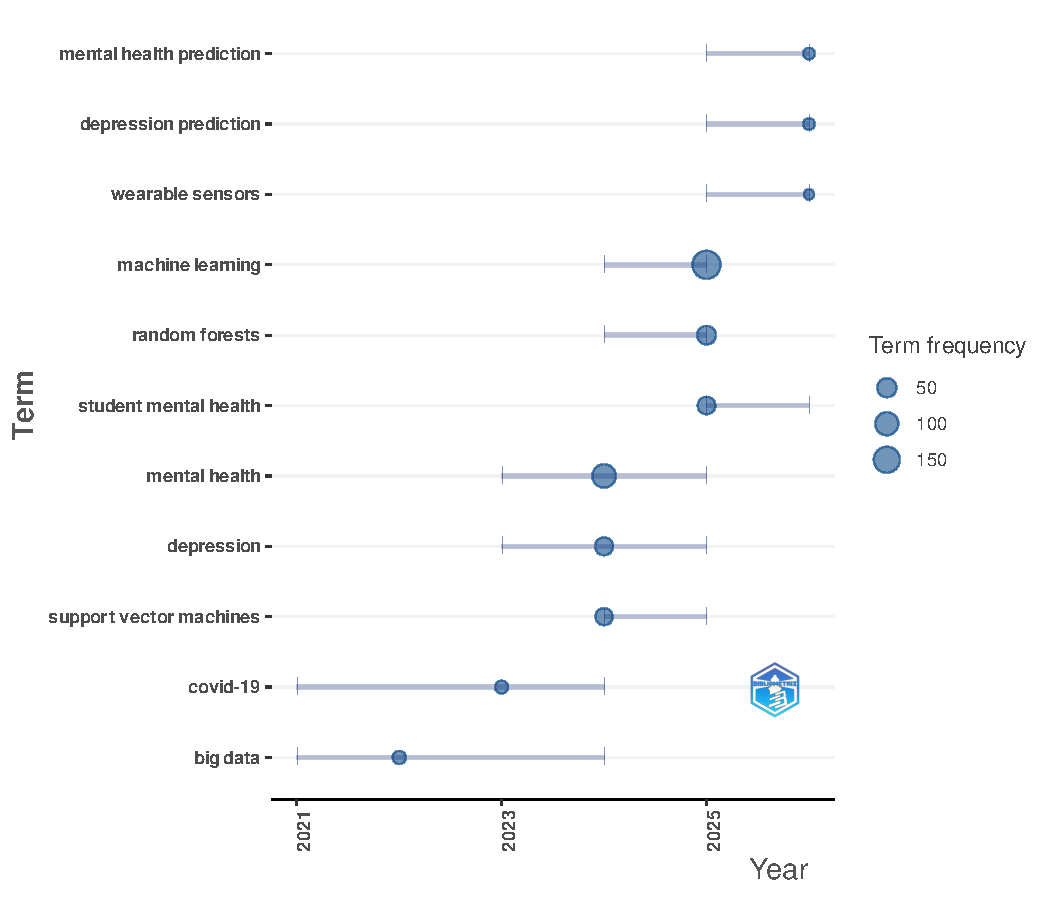
\includegraphics[width=0.75\textwidth]{ieee/en/07_trend_topics}
\caption{IEEE Xplore: trend topics by median year of use.}
\label{fig:ieee-trend}
\end{figure}

\subsection{ScienceDirect}

ScienceDirect contributes 33 included documents (28 journal articles and 5 conference papers). The keyword analysis uses OpenAlex concepts (33 of 33 documents), which are assigned automatically and describe disciplines; they are not directly comparable with author keywords.

\paragraph{Annual production.} Production rose from 2 documents in 2022 to 10 in 2025, and the 10 documents of the partial year 2026 already equal 2025 (Figure~\ref{fig:sd-prod}). No 2021 record was included: the four 2021 records retrieved were unrelated to the topic. The absolute values are small, so a growth rate is not computed.

\paragraph{Sources.} The 33 documents appear in 17 sources, and the three most productive hold 15 documents (45\%) (Figure~\ref{fig:sd-sources}). They represent three areas: psychology (Acta Psychologica, 6), computing (Procedia Computer Science, 5) and multidisciplinary science (Heliyon, 4). Sources are much less dispersed than in IEEE Xplore.

\paragraph{Countries.} 32 documents have a country. China leads with 8 documents, followed by Bangladesh (5), India (4), the United States (3) and Spain (3) (Figure~\ref{fig:sd-countries}). Three European countries (Spain, Italy and Belgium) appear among the ten most productive, while none appears among the ten most productive in IEEE Xplore. Only 3 documents (9\%) have authors from more than one country. The counts are small and should be read as indicative.

\paragraph{Keywords.} The most frequent concepts are computer science and psychology (17 documents each, 52\%), followed by machine learning (14), mental health (13), artificial intelligence (12) and psychiatry (11) (Figure~\ref{fig:sd-keywords}). The profile is the intersection of computing and psychology. In the 86 records retrieved before screening, medicine appeared in 20 documents and psychiatry in 18; among the 33 included documents they appear in 6 and 11. Much of the apparent medical profile of this database therefore came from records unrelated to students.

\paragraph{Excluded charts.} The co-occurrence network, the thematic map and the trend topics are not included. With 33 documents the central nodes of the network overlap, several OpenAlex concepts are disambiguation errors (for example ``classifier (UML)'' or ``feature (linguistics)''), and several themes rest on very few occurrences.

\begin{figure}[htbp]
\centering
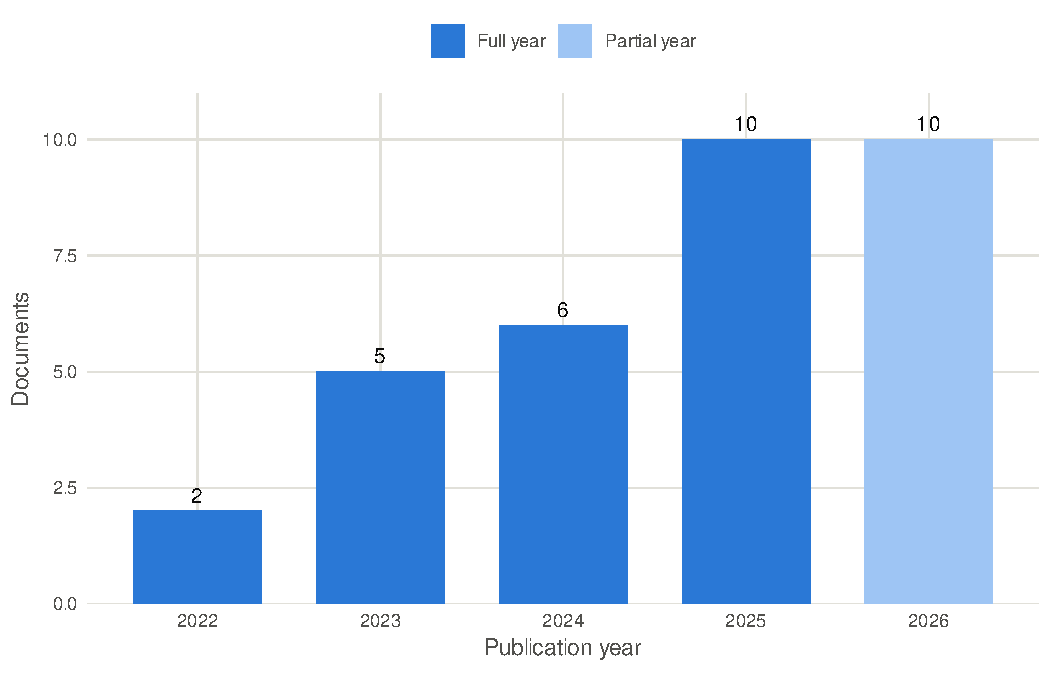
\includegraphics[width=0.7\textwidth]{sciencedirect/en/01_annual_production}
\caption{ScienceDirect: annual scientific production of included documents (2026 is a partial year).}
\label{fig:sd-prod}
\end{figure}

\begin{figure}[htbp]
\centering
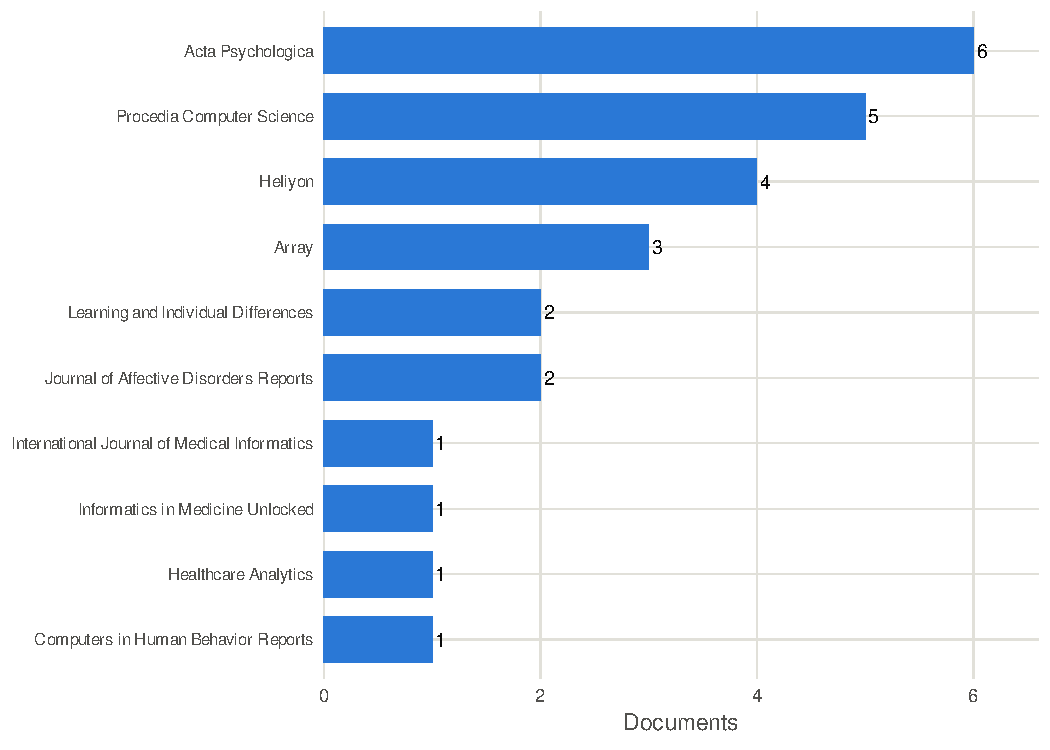
\includegraphics[width=0.8\textwidth]{sciencedirect/en/02_sources}
\caption{ScienceDirect: ten most relevant sources.}
\label{fig:sd-sources}
\end{figure}

\begin{figure}[htbp]
\centering
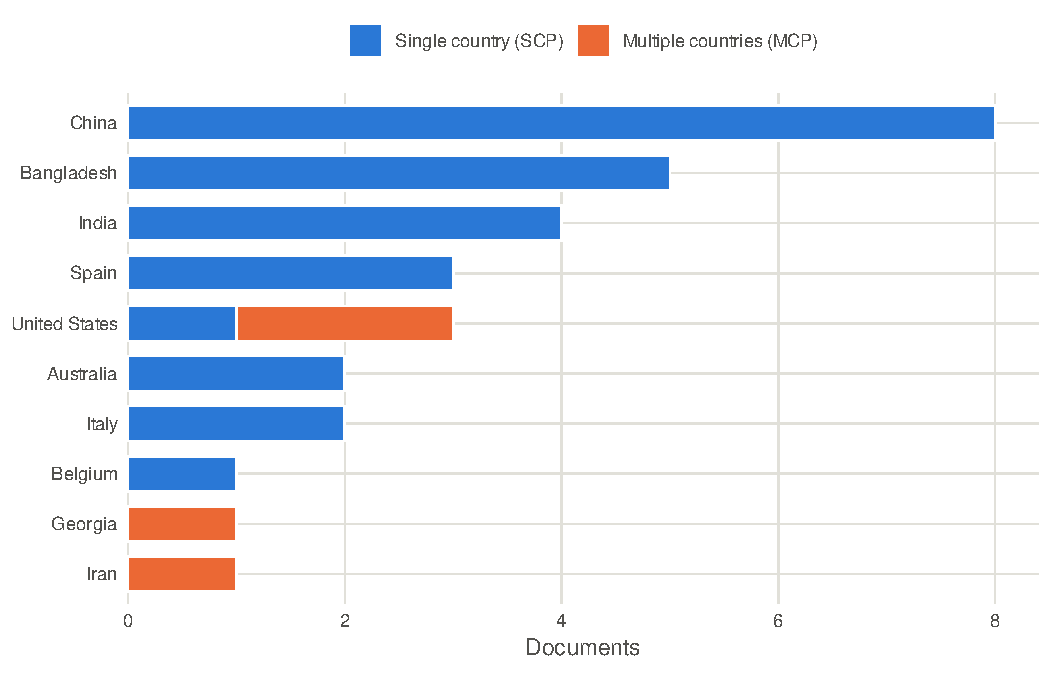
\includegraphics[width=0.7\textwidth]{sciencedirect/en/03_countries}
\caption{ScienceDirect: most productive countries (all authors, full counting).}
\label{fig:sd-countries}
\end{figure}

\begin{figure}[htbp]
\centering
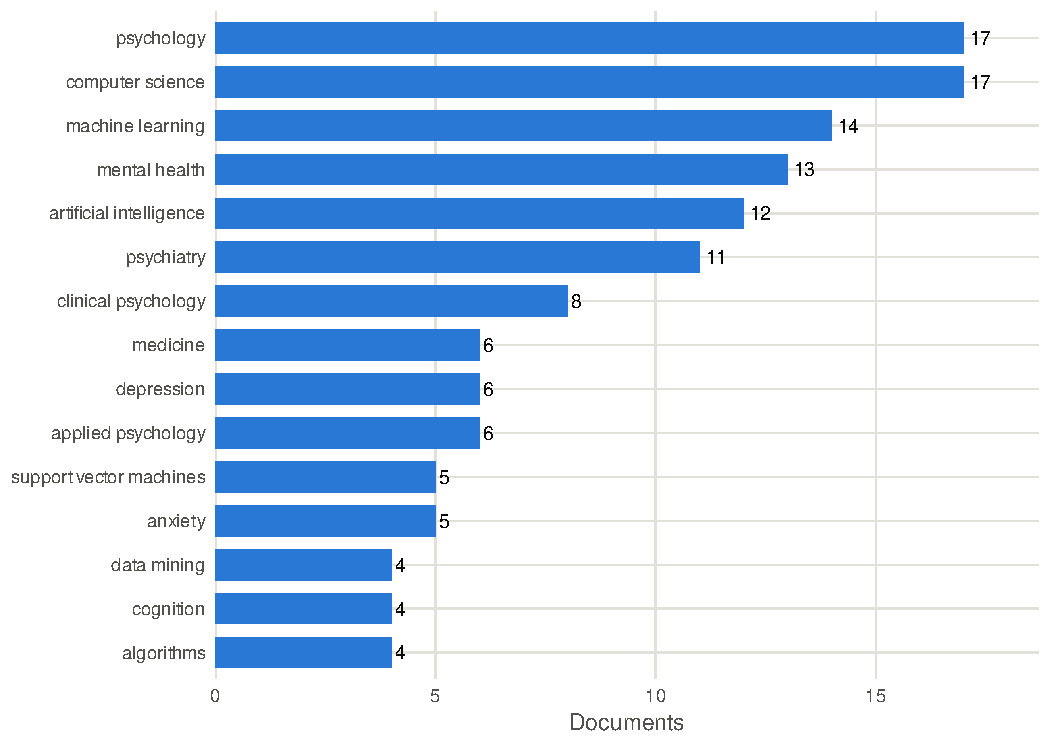
\includegraphics[width=0.7\textwidth]{sciencedirect/en/04_keywords}
\caption{ScienceDirect: most frequent OpenAlex concepts.}
\label{fig:sd-keywords}
\end{figure}

\subsection{SpringerLink}

SpringerLink contributes 43 included documents (19 journal articles and 24 conference papers), all with author keywords. Because SpringerLink was searched in the keyword field, every document contains search terms among its keywords by construction.

\paragraph{Annual production.} Production grows every year: 1 document in 2021 and in 2022, 4 in 2023, 7 in 2024 and 12 in 2025 (Figure~\ref{fig:sl-prod}). The 18 documents of the partial year 2026 already exceed 2025. A growth rate is not computed because a starting value of one document gives a meaningless figure.

\paragraph{Countries.} 36 documents have a country. China accounts for almost half of them (17 documents, 47\%), followed by India (5) and the United States (4) (Figure~\ref{fig:sl-countries}). The share of multiple-country documents (8 of 36, 22\%) is the highest of the three databases; the United States, Hong Kong, Bangladesh and Canada publish mainly in collaboration. Mexico (2 documents) is the only Latin American country among the ten most productive.

\paragraph{Keywords.} Machine learning appears in 63\% of the documents (27 of 43) and mental health in 18, partly because the search was performed on this field (Figure~\ref{fig:sl-keywords}). The distinctive feature of this database is the vocabulary of positive well-being: student well-being (4), subjective well-being (4) and eudaimonic well-being (2).

\paragraph{Co-occurrence network.} The network has three clusters (Figure~\ref{fig:sl-network}). The red cluster links machine learning and mental health with university and college students, depression and early detection. The green cluster groups subjective and eudaimonic well-being, life satisfaction and PISA 2018, and connects to machine learning only through weak links. The blue cluster, student well-being with learning analytics, is isolated from the rest. In this database, positive well-being is studied in parallel with the prediction of mental health problems, not integrated with it.

\paragraph{Excluded charts.} The sources chart, the thematic map and the trend topics are not included. The 43 documents are spread over 35 sources and no source has more than 4 documents; most themes in the thematic map rest on two occurrences of a term, and there are too few repeated terms per year for reliable trends.

\begin{figure}[htbp]
\centering
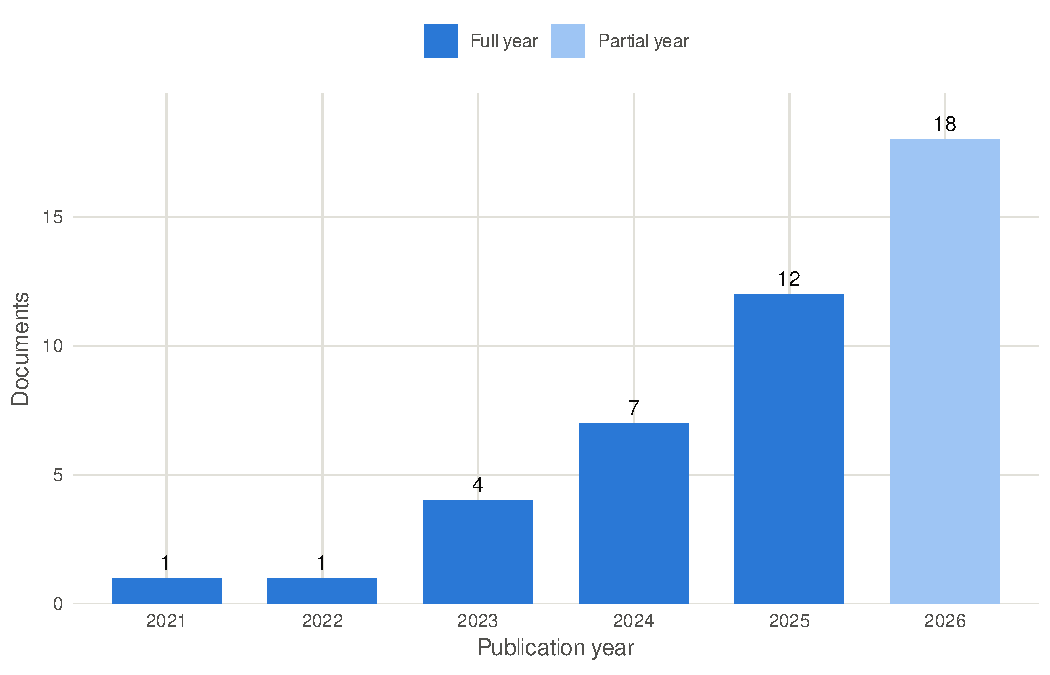
\includegraphics[width=0.7\textwidth]{springerlink/en/01_annual_production}
\caption{SpringerLink: annual scientific production of included documents (2026 is a partial year).}
\label{fig:sl-prod}
\end{figure}

\begin{figure}[htbp]
\centering
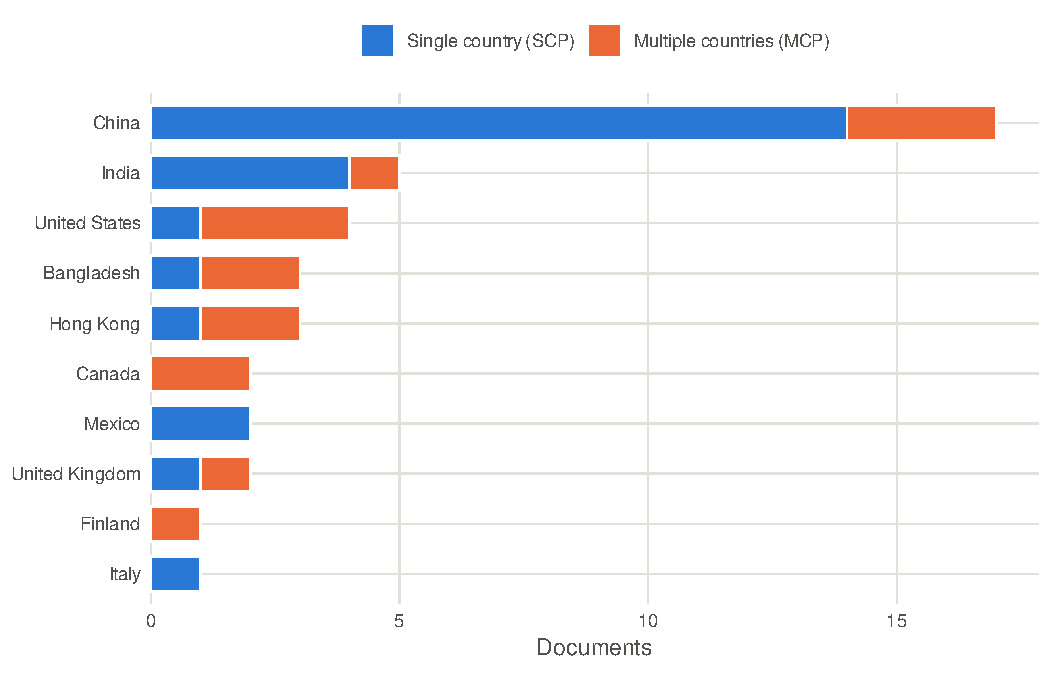
\includegraphics[width=0.7\textwidth]{springerlink/en/03_countries}
\caption{SpringerLink: most productive countries (all authors, full counting).}
\label{fig:sl-countries}
\end{figure}

\begin{figure}[htbp]
\centering
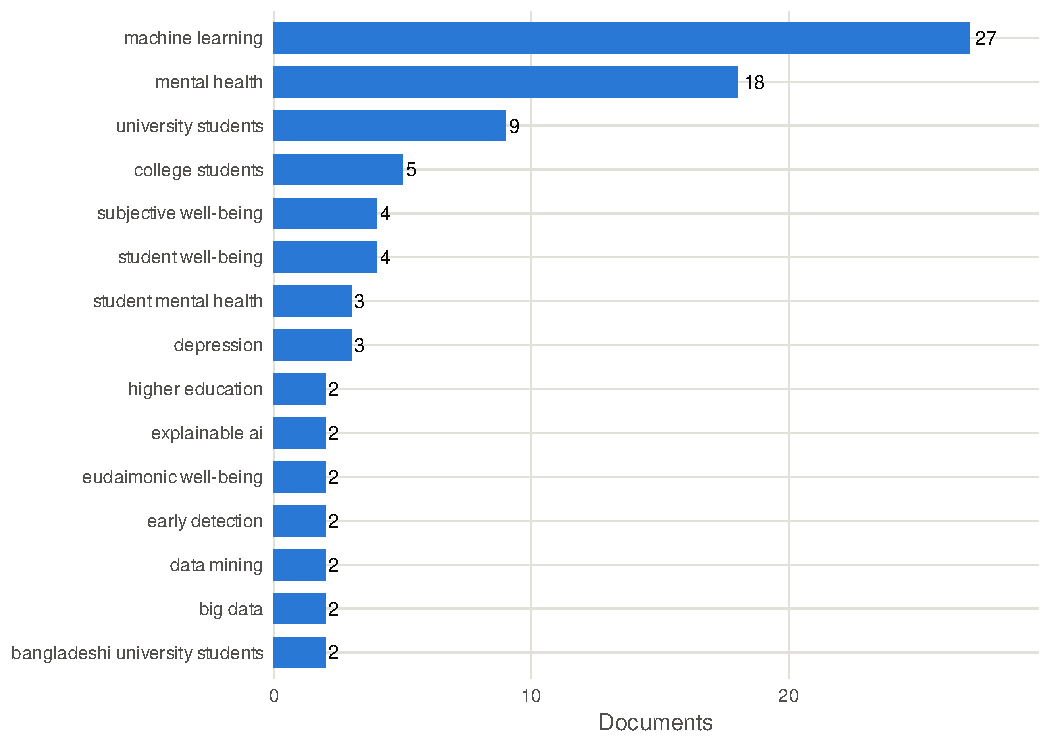
\includegraphics[width=0.7\textwidth]{springerlink/en/04_keywords}
\caption{SpringerLink: most frequent author keywords.}
\label{fig:sl-keywords}
\end{figure}

\begin{figure}[htbp]
\centering
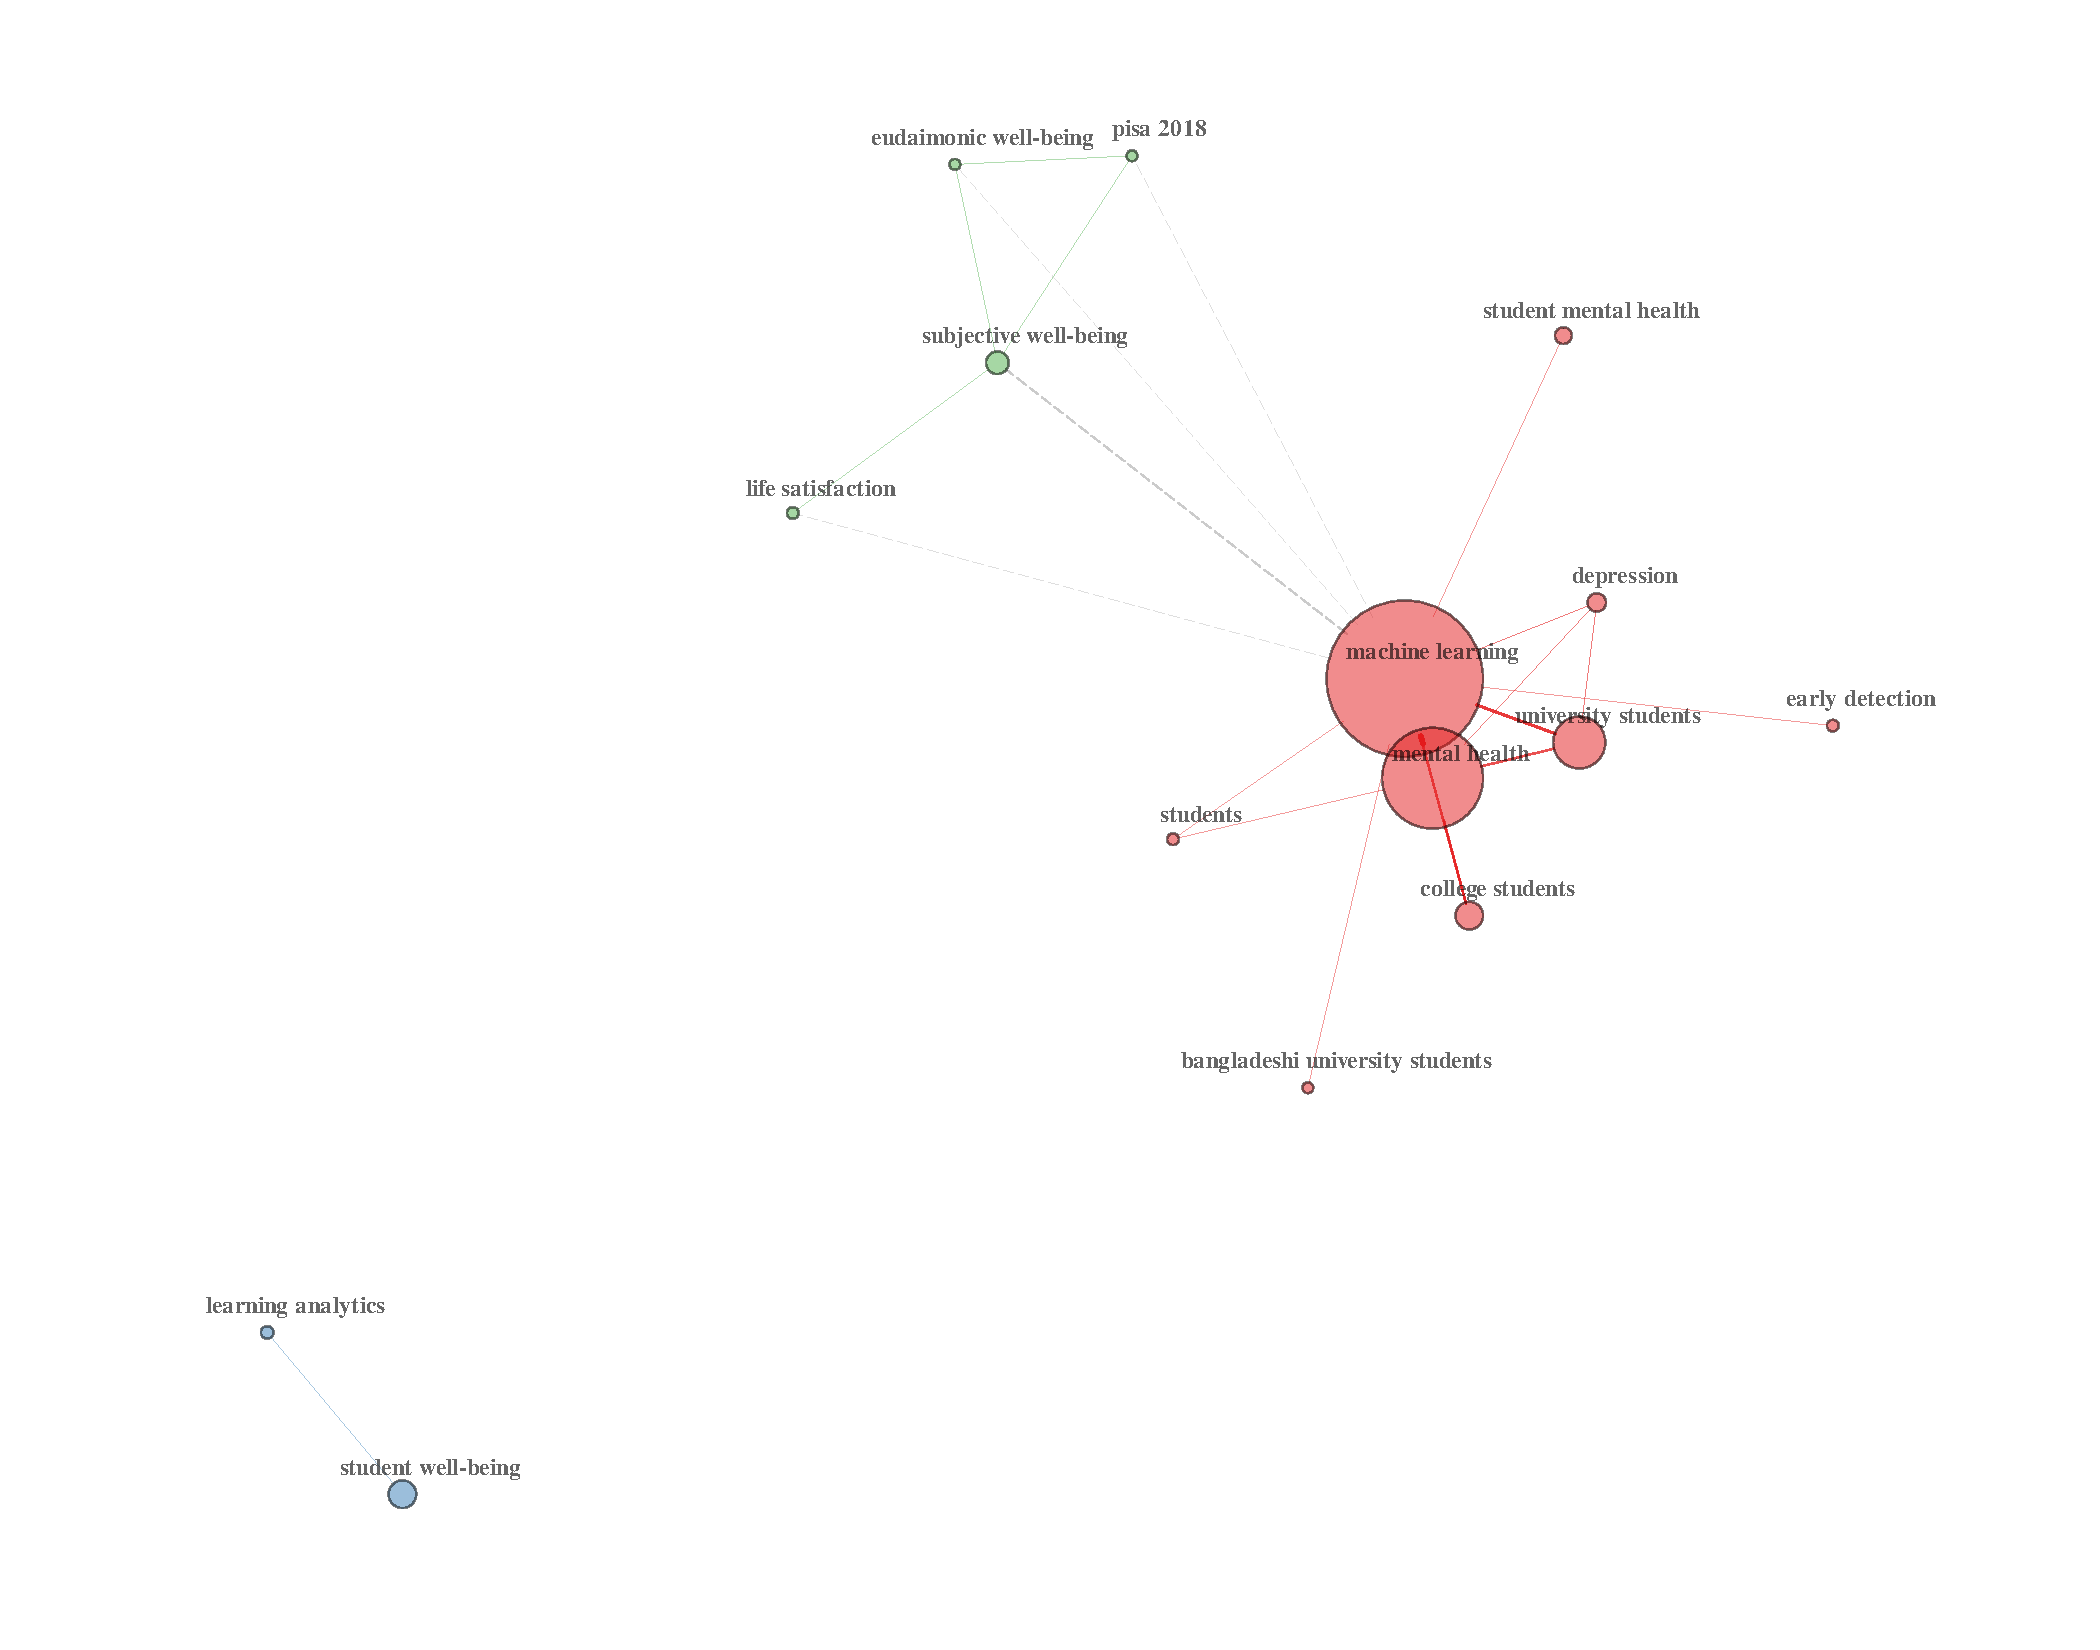
\includegraphics[width=0.9\textwidth]{springerlink/en/05_cooccurrence_network}
\caption{SpringerLink: co-occurrence network of author keywords (Louvain clusters).}
\label{fig:sl-network}
\end{figure}

% =====================================================================
\section{Comparison Between Databases}\label{sec:comparison}

Table~\ref{tab:comparison} summarises the main indicators. Production grows in the three databases, but they differ in volume, document type, geography and thematic emphasis. IEEE Xplore concentrates the work on predictive models, mostly in conference papers. ScienceDirect, once unrelated records are removed, reflects the intersection of psychology and computing in journals. SpringerLink adds the perspective of positive well-being. Bibliographic databases differ in the disciplines they cover \cite{mongeon2016coverage}, and the three databases were searched in different fields, so these differences also reflect the databases and the search, not only the research field.

\begin{table}[htbp]
\centering
\caption{Main indicators of the included documents by database.}
\label{tab:comparison}
\small
\begin{tabularx}{\textwidth}{lYYY}
\toprule
Indicator & IEEE Xplore & ScienceDirect & SpringerLink \\
\midrule
Records screened / included & 933 / 426 (46\%) & 86 / 33 (38\%) & 53 / 43 (81\%) \\
Journal articles / conference papers & 21 / 405 & 28 / 5 & 19 / 24 \\
Production 2021 $\rightarrow$ 2025 & 25 $\rightarrow$ 160 (CAGR 59.1\%) & 0 $\rightarrow$ 10 & 1 $\rightarrow$ 12 \\
Distinct sources & 342 & 17 & 35 \\
Leading countries & India 153, China 94, Bangladesh 38 & China 8, Bangladesh 5, India 4 & China 17, India 5, United States 4 \\
Multiple-country documents & 11.7\% & 9.4\% & 22.2\% \\
Keyword field & Author keywords & OpenAlex concepts & Author keywords \\
Distinctive themes & Classical classifiers, deep learning, XAI, NLP & Psychology and computing & Subjective and eudaimonic well-being \\
Vague abstracts & 43\% & 9\% & 21\% \\
XAI reported & 10\% & 33\% & 23\% \\
\bottomrule
\end{tabularx}
\end{table}

% =====================================================================
\section{Discussion}\label{sec:discussion}

\subsection{Answers to the research questions}

\textbf{RQ1 (evolution).} Production grew in the three databases between 2021 and 2025, at a compound annual rate of 59.1\% in IEEE Xplore. With 2026 still incomplete, its production already exceeds that of 2023 in IEEE Xplore (70 versus 50), equals 2025 in ScienceDirect (10) and exceeds 2025 in SpringerLink (18 versus 12).

\textbf{RQ2 (countries).} India, China and Bangladesh lead the production. The countries stated in the abstracts point in the same direction: Bangladesh (27 studies), China (20) and India (17) are the most frequent. International collaboration is low (between 9.4\% and 22.2\% of the documents), and the two most productive countries publish almost entirely without foreign partners. Latin America is marginal (Peru and Mexico).

\textbf{RQ3 (sources).} The research is published mainly in conference proceedings and is highly dispersed, especially in IEEE Xplore, where 342 sources share 426 documents. Only ScienceDirect shows some concentration in journals (Acta Psychologica, Procedia Computer Science, Heliyon).

\textbf{RQ4 (outcomes, populations, data and techniques).} The field is organised around predicting stress, depression and anxiety in university students, mostly from questionnaires and with classical classifiers and tree ensembles. Sensor-based, text-based and multimodal approaches form secondary lines. Suicide, secondary school students and positive well-being receive comparatively little attention.

\textbf{RQ5 (change over time).} The vocabulary moves from context terms (big data, COVID-19) towards prediction and, most recently, towards prediction with wearable sensors. The coded content shows the same direction: the share of studies using deep learning and XAI increased, and XAI rose from 4\% to 32\%.

\textbf{RQ6 (database emphasis).} IEEE Xplore shows predictive modelling, ScienceDirect the intersection of psychology and computing, and SpringerLink positive well-being. Because IEEE Xplore provides 85\% of the included documents, the general conclusions mainly reflect that database.

\subsection{Gaps}

The main gap is methodological. Validation on an external cohort is reported in only two abstracts, calibration in three and fairness in seven, while at least 44 studies report performance values of 98\% or more. Small samples with inadequate validation inflate performance estimates \cite{vabalas2019validation}, and information leakage is a frequent cause of irreproducible results \cite{kapoor2023leakage}. No abstract mentions a reporting guideline such as TRIPOD+AI \cite{collins2024tripodai}, and 26\% of the abstracts do not state the data used.

The use of XAI is growing, but explaining a complex model after training is not equivalent to using a model that is interpretable by design, and for high-stakes decisions interpretable models are preferable \cite{rudin2019blackbox}. Screening students for mental health problems is a high-stakes decision: a false negative can leave a student at risk without support, which is why some studies in the corpus prioritise recall \cite{S008}.

Thematically, positive well-being and the prediction of mental health problems are studied in parallel, as the SpringerLink network shows. Suicide appears in only 3\% of the studies and secondary school students in 5\%. Privacy or confidentiality is mentioned in 39 abstracts (8\%), usually as a design feature or an ethical concern rather than as the subject of the study.

\subsection{Future research agenda}

Based on these gaps, future research should: (i) validate models on independent datasets, across institutions and over time; (ii) report studies following TRIPOD+AI \cite{collins2024tripodai}, including the data source, sample size, handling of class imbalance and calibration; (iii) prefer interpretable models or evaluate explanations with their users, such as counsellors; (iv) connect positive well-being constructs with the prediction of mental health problems; (v) evaluate whether early warning systems improve student outcomes, not only whether they classify accurately; (vi) address fairness, consent and privacy explicitly; and (vii) extend the evidence to secondary education and to regions with little presence in the corpus, such as Latin America.

% =====================================================================
\section{Limitations}\label{sec:limitations}

This study has several limitations. First, the corpus comes from three databases accessed through their APIs with different search fields: SpringerLink was searched only in keywords, and ScienceDirect records were retrieved through Scopus. Relevant studies indexed elsewhere, or described only in the full text, may be missing. Second, the databases are unbalanced: IEEE Xplore provides 85\% of the included documents. Third, screening and data extraction were based on abstracts only and were carried out with the assistance of a large language model under a closed codebook, followed by checks on random samples, targeted checks of doubtful decisions and documented harmonisation rules; a full independent double coding by human reviewers was not performed. Fourth, the APIs do not provide reference lists, so citation-based analyses (co-citation, bibliographic coupling, most cited references) were not possible. Fifth, ScienceDirect keywords are automatically assigned OpenAlex concepts, which are not comparable with author keywords and contain disambiguation errors. Sixth, 2026 is a partial year, and citation counts and OpenAlex fields change over time; all results refer to the snapshot of 28 September 2026. Finally, only English-language records were analysed.

% =====================================================================
\section{Conclusions}\label{sec:conclusions}

This study combined a systematic review of 502 abstracts with a comparative bibliometric analysis of IEEE Xplore, ScienceDirect and SpringerLink to map student well-being and mental health analytics between 2021 and 2026. The field is growing quickly and is concentrated in India, China and Bangladesh. It is organised around the prediction of stress, depression and anxiety in university students from questionnaires with classical classifiers and tree ensembles, and it is moving towards deep learning, language models, wearable sensors and explainable models.

Screening the abstracts changed the picture: almost one third of the retrieved records were unrelated to the topic, and removing them changed the apparent profile of ScienceDirect. The main weakness of the field is the gap between the high performance that studies report and the weak validation behind it. Progress now depends on validation on independent data, transparent reporting, interpretable models and evidence that early warning systems help students.

% =====================================================================
\section*{Declarations}

\paragraph{Data availability.} The search equations, retrieval and analysis scripts, codebook, coded screening records (with record identifiers and DOIs) and harmonisation log are openly available at \url{https://github.com/lyc4nthrope/student-wellbeing-mental-health-analytics-review}. Publisher abstracts are not redistributed; they can be retrieved again with the retrieval script and the reader's own API keys.

\paragraph{Use of artificial intelligence.} A large language model was used to assist abstract screening, data extraction and the drafting of this manuscript. The author reviewed the outputs and is responsible for the content.

\bibliographystyle{unsrtnat}
\bibliography{references,corpus}

\end{document}
